\documentclass[tikz,border=5pt]{standalone}
\usepackage{tkz-euclide}
\begin{document}
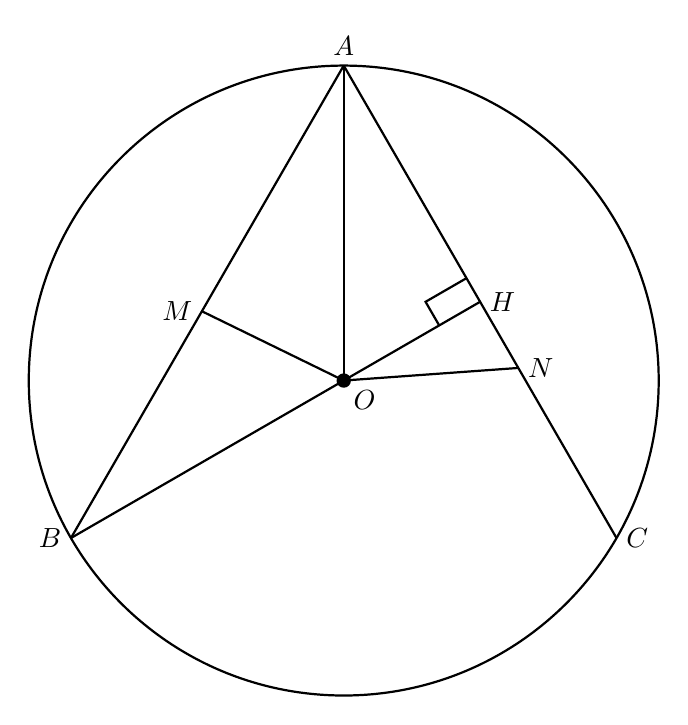
\begin{tikzpicture}[scale=1]

% Circle and main points
\def\R{4}
\coordinate (O) at (0,0);
\coordinate (A) at (90:\R);
\coordinate (B) at (210:\R);
\coordinate (C) at (330:\R);

% Auxiliary points on sides
\coordinate (M) at ($(A)!0.52!(B)$);
\coordinate (N) at ($(A)!0.64!(C)$);

% Foot from B to AC
\coordinate (H) at ($(A)!(B)!(C)$);

% Circle
\draw[line width=0.8pt] (O) circle (\R);

% Triangle sides
\draw[line width=0.8pt] (A)--(B);
\draw[line width=0.8pt] (A)--(C);

% Interior segments
\draw[line width=0.8pt] (A)--(O);
\draw[line width=0.8pt] (M)--(O);
\draw[line width=0.8pt] (O)--(N);

% Added perpendicular from B to AC
\draw[line width=0.8pt] (B)--(H);

% Right angle mark at H
\draw[line width=0.8pt]
  ($(H)!0.10!(A)$) --
  ($($(H)!0.10!(A)$)+($(H)!0.10!(B)$)-(H)$) --
  ($(H)!0.10!(B)$);

% Point O
\fill (O) circle (2.6pt);

% Labels
\node[above] at (A) {$A$};
\node[left] at (B) {$B$};
\node[right] at (C) {$C$};
\node[left] at (M) {$M$};
\node[right] at (N) {$N$};
\node[below right] at (O) {$O$};
\node[right] at (H) {$H$};

\end{tikzpicture}
\end{document}
